%% ----------------------------------------------------------------
%% Thesis.tex -- MAIN FILE (the one that you compile with LaTeX)
%% ---------------------------------------------------------------- 

% Set up the document
\documentclass[a4paper, oneside]{Thesis}  % Use the "Thesis" style, based on the ECS Thesis style by Steve Gunn
\graphicspath{{Figures/}}  % Location of the graphics files (set up for graphics to be in PDF format)

% Include any extra LaTeX packages required
\usepackage[square, numbers, comma, sort&compress]{natbib}  % Use the "Natbib" style for the references in the Bibliography
\usepackage{verbatim}  % Needed for the "comment" environment to make LaTeX comments
\usepackage{vector}  % Allows "\bvec{}" and "\buvec{}" for "blackboard" style bold vectors in maths
\hypersetup{urlcolor=blue, colorlinks=true}  % Colours hyperlinks in blue, but this can be distracting if there are many links.
\usepackage{makeidx}

% The following is needed in order to make the code compatible
% with both latex/dvips and pdflatex.
\ifx\pdftexversion\undefined
\usepackage[dvips]{graphicx}
\else
%\usepackage[pdftex]{graphicx}
\DeclareGraphicsRule{*}{mps}{*}{}
\fi

\usepackage{multicol}
\usepackage{float}
\usepackage{listings}
\usepackage{color}
\usepackage{ifthen}
\usepackage[table,x11name,rgb]{xcolor}
\usepackage{textcomp}
\usepackage{alltt}
\usepackage[utf8]{inputenc}
\usepackage[utf8]{vietnam}
\usepackage{mathptmx}
\usepackage[scaled=.90]{helvet}
\usepackage{courier}
\usepackage{sectsty}
\usepackage{amssymb}
%\usepackage[titles]{tocloft}
\usepackage[subfigure]{tocloft}
%\usepackage{doxygen}
%\usepackage{pgf-umlsd}
%\usepackage{minted}
\usepackage{xparse}
\usepackage{tikz}
\usetikzlibrary{snakes,arrows,shapes}
\usepackage{tikz-uml}
\usepackage{amsmath}
\lstset{language=C++,inputencoding=utf8,basicstyle=\footnotesize,breaklines=true,breakatwhitespace=true,tabsize=4,numbers=left }
\makeindex
\setcounter{tocdepth}{3}
\renewcommand{\footrulewidth}{0.4pt}
\renewcommand{\familydefault}{\sfdefault}
\hfuzz=15pt
\setlength{\emergencystretch}{15pt}
\hbadness=750
\tolerance=750
\newcommand{\executeiffilenewer}[3]{%
    \ifnum\pdfstrcmp{\pdffilemoddate{#1}}%
    {\pdffilemoddate{#2}}>0%
    {\immediate\write18{#3}}\fi%
}
\newcommand{\includesvg}[1]{%
    \executeiffilenewer{#1.svg}{#1.pdf}%
    {inkscape -z -D --file=#1.svg %
        --export-pdf=#1.pdf --export-latex}%
    \input{#1.pdf_tex}%
}


%% ----------------------------------------------------------------
\begin{document}
\frontmatter	  % Begin Roman style (i, ii, iii, iv...) page numbering

% Set up the Title Page
\title  {Báo cáo môn học Nhập môn công nghệ phần mềm}
\authors {
    {Trịnh Hoàng Hà - 20101461}{} \\
    {Tạ Văn Trường - 20102404}\\
    {Nguyễn Duy Thành - 20102737}{} \\
}
\supervisor  {Lương Mạnh Bá}
\UNIVERSITY {\texorpdfstring{\href{http://hut.edu.vn/}
                {ĐẠI HỌC BÁCH KHOA HÀ NỘI}}
                {ĐẠI HỌC BÁCH KHOA HÀ NỘI}}
\department  {\texorpdfstring{\href{http://soict.hut.edu.vn}
                {Bộ môn Công nghệ phần mềm}}
                {Bộ môn Công nghệ phần mềm}}
\group       {\texorpdfstring{\href{Research Group Web Site URL Here (include http://)}
                {Nhóm 40 - K55}}
                {Nhóm 40 - K55}}
\faculty     {\texorpdfstring{\href{Faculty Web Site URL Here (include http://)}
                {Viện công nghệ thông tin và truyền thông}}
                {Viện công nghệ thông tin và truyền thông}}
\addresses  {\groupname\\\deptname\\\univname}  % Do not change this here, instead these must be set in the "Thesis.cls" file, please look through it instead
\date       {\today}
\subject    {Quy trình phát triển phần mềm nhúng}
\keywords   {}

\maketitle
%% ----------------------------------------------------------------

\setstretch{1.3}  % It is better to have smaller font and larger line spacing than the other way round

% Define the page headers using the FancyHdr package and set up for one-sided printing
\fancyhead{}  % Clears all page headers and footers
\rhead{\thepage}  % Sets the right side header to show the page number
\lhead{}  % Clears the left side page header

\pagestyle{fancy}  % Finally, use the "fancy" page style to implement the FancyHdr headers

%% ----------------------------------------------------------------
% Declaration Page required for the Thesis, your institution may give you a different text to place here
%\Declaration{
%
%\addtocontents{toc}{\vspace{1em}}  % Add a gap in the Contents, for aesthetics
%
%I, AUTHOR NAME, declare that this thesis titled, `THESIS TITLE' and the work presented in it are my own. I confirm that:
%
%\begin{itemize} 
%\item[\tiny{$\blacksquare$}] This work was done wholly or mainly while in candidature for a research degree at this University.
% 
%\item[\tiny{$\blacksquare$}] Where any part of this thesis has previously been submitted for a degree or any other qualification at this University or any other institution, this has been clearly stated.
% 
%\item[\tiny{$\blacksquare$}] Where I have consulted the published work of others, this is always clearly attributed.
% 
%\item[\tiny{$\blacksquare$}] Where I have quoted from the work of others, the source is always given. With the exception of such quotations, this thesis is entirely my own work.
% 
%\item[\tiny{$\blacksquare$}] I have acknowledged all main sources of help.
% 
%\item[\tiny{$\blacksquare$}] Where the thesis is based on work done by myself jointly with others, I have made clear exactly what was done by others and what I have contributed myself.
%\\
%\end{itemize}
% 
% 
%Signed:\\
%\rule[1em]{25em}{0.5pt}  % This prints a line for the signature
% 
%Date:\\
%\rule[1em]{25em}{0.5pt}  % This prints a line to write the date
%}
%\clearpage  % Declaration ended, now start a new page

%% ----------------------------------------------------------------
% The "Funny Quote Page"
%\pagestyle{empty}  % No headers or footers for the following pages
%
%\null\vfill
%% Now comes the "Funny Quote", written in italics
%\textit{``Write a funny quote here.''}
%
%\begin{flushright}
%If the quote is taken from someone, their name goes here
%\end{flushright}
%
%\vfill\vfill\vfill\vfill\vfill\vfill\null
%\clearpage  % Funny Quote page ended, start a new page
%%% ----------------------------------------------------------------
%
% The Abstract Page
\addtotoc{Lời nói đầu}  % Add the "Abstract" page entry to the Contents
\abstract{
\addtocontents{toc}{\vspace{1em}}  % Add a gap in the Contents, for aesthetics

Hiện nay, đến 99\% số máy tính (thiết bị tính toán có sử dụng vi xử lý)
    được bán ra hàng năm là máy tính nhúng, trong khi PC chỉ chiếm 1\% còn lại.
    Như vậy, rõ ràng nhu cầu về phần mềm nhúng là rất lớn. Tuy nhiên, do những
    đặc điểm riêng của phần mềm nhúng cũng như hệ thống nhúng mà việc phát
    triển phần mềm nhúng có nhiều khác biệt so với phần mềm trên PC (thường
    là khó hơn).
    
    Nhóm chúng em chọn đề tài này để tìm hiểu về quy trình phát triển phần mềm
    nhúng, nhằm tìm ra những điểm khác biệt, những khó khăn trong việc phát
    triển phần mềm nhúng so với phần mềm thông thường và nêu một số giải pháp.
    Qua đó có thể áp dụng được cho các công việc trong tương lai.

    Trước khi bắt đầu đề tài của mình chúng em xin được bày tỏ lòng cảm ơn tới
    các thầy đã hết lòng, hết sức giảng dạy cho chúng em trong suốt thời gian
    qua và đặc biệt là với Thầy Lương Mạnh Bá là người đã trực tiếp giảng dạy
    và hướng dẫn chúng em thực hiện đề tài này.
}

\clearpage  % Abstract ended, start a new page
%% ----------------------------------------------------------------

\setstretch{1.3}  % Reset the line-spacing to 1.3 for body text (if it has changed)

% The Acknowledgements page, for thanking everyone
%\acknowledgements{
%\addtocontents{toc}{\vspace{1em}}  % Add a gap in the Contents, for aesthetics
%
%The acknowledgements and the people to thank go here, don't forget to include your project advisor\ldots
%
%}
\clearpage  % End of the Acknowledgements
%% ----------------------------------------------------------------

\pagestyle{fancy}  %The page style headers have been "empty" all this time, now use the "fancy" headers as defined before to bring them back


%% ----------------------------------------------------------------
\lhead{\emph{Contents}}  % Set the left side page header to "Contents"
\tableofcontents  % Write out the Table of Contents

%% ----------------------------------------------------------------
\lhead{\emph{List of Figures}}  % Set the left side page header to "List if Figures"
\listoffigures  % Write out the List of Figures

%% ----------------------------------------------------------------
\lhead{\emph{List of Tables}}  % Set the left side page header to "List of Tables"
\listoftables  % Write out the List of Tables

%% ----------------------------------------------------------------
\setstretch{1.5}  % Set the line spacing to 1.5, this makes the following tables easier to read
\clearpage  % Start a new page
\lhead{\emph{Abbreviations}}  % Set the left side page header to "Abbreviations"
\listofsymbols{ll}  % Include a list of Abbreviations (a table of two columns)
{
\textbf{DFD} & \textbf{D}ata \textbf{F}low \textbf{D}iagram: Đồ thị luồng dữ
liệu \\
\textbf{ROOM} & \textbf{R}eal-time \textbf{O}bject \textbf{O}riented Modeling:
Mô hình hướng đối tượng thời gian thực \\
\textbf{UML} & \textbf{U}nified \textbf{M}odeling \textbf{L}anguage: Ngôn ngữ
mô hình hoá thống nhất \\
}

%% ----------------------------------------------------------------
%\clearpage  % Start a new page
%\lhead{\emph{Physical Constants}}  % Set the left side page header to "Physical Constants"
%\listofconstants{lrcl}  % Include a list of Physical Constants (a four column table)
%{
%% Constant Name & Symbol & = & Constant Value (with units) \\
%Speed of Light & $c$ & $=$ & $2.997\ 924\ 58\times10^{8}\ \mbox{ms}^{-\mbox{s}}$ (exact)\\
%
%}

%% ----------------------------------------------------------------
%\clearpage  %Start a new page
%\lhead{\emph{Symbols}}  % Set the left side page header to "Symbols"
%\listofnomenclature{lll}  % Include a list of Symbols (a three column table)
%{
%% symbol & name & unit \\
%$a$ & distance & m \\
%$P$ & power & W (Js$^{-1}$) \\
%& & \\ % Gap to separate the Roman symbols from the Greek
%$\omega$ & angular frequency & rads$^{-1}$ \\
%}
%% ----------------------------------------------------------------
% End of the pre-able, contents and lists of things
% Begin the Dedication page

%\setstretch{1.3}  % Return the line spacing back to 1.3

%\pagestyle{empty}  % Page style needs to be empty for this page
%\dedicatory{For/Dedicated to/To my\ldots}

%\addtocontents{toc}{\vspace{2em}}  % Add a gap in the Contents, for aesthetics


%% ----------------------------------------------------------------
\mainmatter	  % Begin normal, numeric (1,2,3...) page numbering
\pagestyle{fancy}  % Return the page headers back to the "fancy" style

\renewcommand{\headrulewidth}{0.5pt}
\renewcommand{\footrulewidth}{0pt}
\renewcommand{\chaptermark}[1]{\markboth{#1}{}}
\renewcommand{\sectionmark}[1]{\markright{#1}{}}
\renewcommand{\chaptermark}[1]{\markboth{\chaptername\ \thechapter.\ #1}{}}

\lhead{\leftmark}

% Include the chapters of the thesis, as separate files
% Just uncomment the lines as you write the chapters

%\input{./Chapters/Chapter5} % Phân công công việc
%\input{./Chapters/Foreword2}
\chapter{Hệ thống nhúng và phần mềm nhúng}

%========== System ======================}
    \section{Hệ thống nhúng}

        \subsection{Định nghĩa}
Hệ thống nhúng(embedded system) là một thuật ngữ để chỉ một hệ thống có khả năng tự trị được nhúng vào trong một môi trường hay một hệ thống mẹ. Đó là  các hệ thống tích hợp cả phần cứng và phần mềm phục vụ các bài toán chuyên dụng trong nhiều lĩnh vực công nghiệp, tự động hóa điều khiển, quan trắc và truyền tin...Đặc điểm của các hệ thống nhúng là hoạt động ổn định và có tính năng tự động hóa cao.

Hệ thống nhúng thường được thiết kế để thực hiện một chức năng chuyên dụng, thường nó có khả năng tự hành và được thiết kế tích hợp vào một hệ thống lớn hơn để thực hiện một chức năng nào đó. Khác với các máy tính đa chức năng, một hệ thống nhúng chỉ thực hiện một hoặc một vài chức năng nhất định, thường đi kèm với những yêu cầu cụ thể và bao gồm một số thiết bị máy móc và phần cứng chuyên dụng mà ta không tìm thấy trong một máy tính đa chức năng nói chung.

Vì hệ thống chỉ được xây dựng cho một số nhiệm vụ nhất định nên cá nhà thiết kế có thể tối ưu hóa nó nhằm giảm thiểu kích thước và chi phí sản xuất. Các hệ thống nhúng thường được sản xuất hàng loạt với số lượng lớn. Hệ thống nhúng rất đa dạng và phong phú về chủng loại. Đó có thể là những thiết bị cầm tay nhỏ gọn như đồng hồ kĩ thuật số, máy chơi nhạc MP3 hoặc những sản phẩm lớn như cột đèn giao thông, bộ kiểm soát trong nhà máy... Xét về độ phức tạp, hệ thống nhúng có thể rất đơn giản với một vi điều khiển hoặc rất phức tạp với nhiều đơn vị, các thiết bị ngoại vi và mạng lưới được nằm gọn trong một lớp vỏ máy lớn. Các thiết bị như máy tính cầm tay cũng có một số đặc điểm tương tự với hệ thống nhúng.
Hệ thống nhúng bao gồm các thiết bị  phần cứng và phần mềm, hầu hết đều phải thỏa mãn yêu cầu hoạt động theo thời gian thực( real- time). Tùy theo tính chất và yêu cầu, mức độ đáp ứng của hệ thống có thẻ rất nhanh hoặc có thể chấp nhận một mức độ chậm chễ nhất định.

        \subsection{Độ tin cậy của hệ thống nhúng}
Các hệ thống nhúng thường nằm trong các cỗ máy được kì vọng là sẽ chạy hàng năm trời liên tục mà không gặp lỗi hoặc có thể khôi phục khi gặp lỗi. Vì thế các phần mềm và hệ thống nhúng được phát triển và kiểm thử một cách cẩn thận hơn là phần mềm cho máy tính cá nhân.

Ngoài ra, các thiết bị rời không đáng tin cậy như ổ đĩa, công tắc hoặc nút bấm thường được hạn chế sử dụng.

Một số vấn đề cụ thể về độ tin cậy như:
            \begin{itemize}
                \item Hệ thống không thể ngừng để sửa chữa một cách an toàn như  các hệ thống không gian, hệ thống dây cáp dưới biển, các đèn hiệu dẫn đường...Giải pháp đưa ra là  chuyển sang sử dụng các hệ thống con dự trữ hoặc các phần mềm cung cấp một phần chức năng.
                \item Hệ thống phải được chạy liên tục vì tính an toàn, ví dụ như các thiết bị dẫn đường máy bay, thiết bị kiểm soát độ an toàn trong các nhà máy hóa chất,… Giải pháp đưa ra là lựa chọn backup hệ thống.
                \item Nếu hệ thống ngừng hoạt động sẽ gây tổn thất rất nhiều tiền của ví dụ như các dịch vụ buôn bán tự động, hệ thống chuyển tiền, hệ thống kiểm soát trong các nhà máy...
            \end{itemize}

%================= Software ==================================
    \section{Phần mềm nhúng}

Là phần mềm trong các hệ thống nhúng. Phần mềm nhúng có thể là những chương trình đơn giản chạy trực tiếp trên nền phần cứng hoặc là những chương trình, ứng dụng chạy trên nền một hệ điều hành nhúng. Phần mềm nhúng thường chạy với số tài nguyên phần cứng hạn chế: không có bàn phím, màn hình hoặc có nhưng với kích thước nhỏ, bộ nhớ hạn chế.

Phần mềm nhúng thường được lập trình trên máy tính cá nhân của lập trình viên, được biên dịch với một trình biên dịch và một môi trường phát triển, máy tính dùng để lập trình được gọi là host. Sau đó chương trình được nạp lên thiết bị và chạy, thiết bị mà chương trình được nạp lên gọi la target.Với mỗi target khác nhau sẽ có cấu trúc vi điểu khiển khác nhau, và sử dụng hệ điều hành nhúng khác nhau, do vậy tùy từng loại sẽ có các cách thức lập trình tương ứng.

    
        
        \begin{figure}[H]
            \centering
            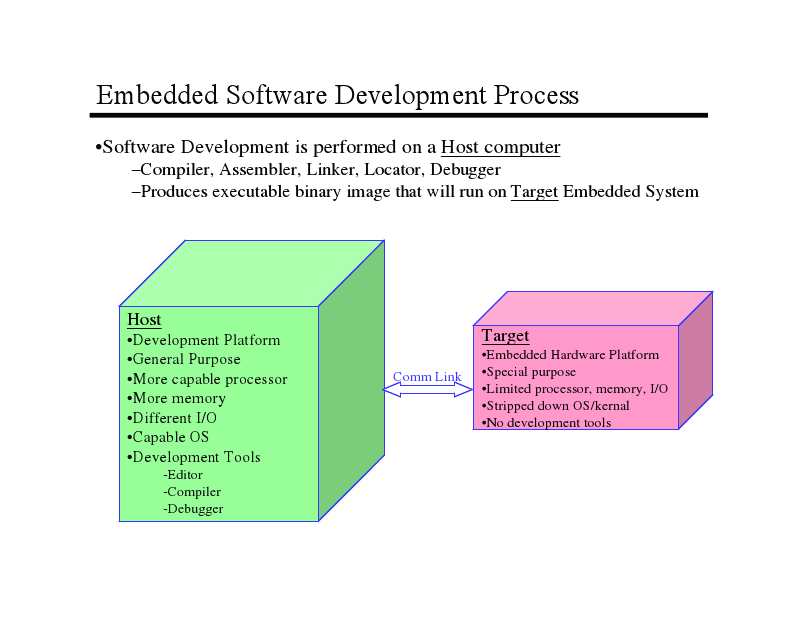
\includegraphics[scale=0.6]{hosttarget}
            \rule{35em}{0.5pt}
            \caption{Host và target trong phát triển phần mềm nhúng}
            \label{fig:hosttarget}
        \end{figure}

    C là một trong những ngôn ngữ lập trình nhúng phổ biến nhất hiện nay. C có một số ưu điểm nổi bật tiêu biểu như khá nhỏ và dễ dàng cho việc học, các chương trình biên dịch C thường khá sẵn cho hầu hết các bộ xử lý đang sử dụng hiện nay, và có rất nhiều người đã biết và làm chủ được ngôn ngữ này. 

 So với phần mềm thông thường, phần mềm nhúng có những điểm khác biệt sau:
    
    \begin{itemize}
        \item Phần mềm và phần cứng được phát triển cùng một lúc,
        \item Máy tính dùng để phát triển phần mềm (host) thường xuyên khác với target,
        \item Phần cứng cho target thường xuyên không có sẵn cho đến gần kết thúc dự án,
        \item Thương không rõ một lỗi nào đó là lỗi phần cứng hay lỗi phần mềm,
        \item Lỗi phần cứng thường được “chữa” bằng phần mềm,
        \item Số tiền bỏ ra cho phát triển phần mềm gấp hàng trăm lần so với phần cứng, do đó phần mềm thường được yêu cầu làm những việc mà nó nên được thực hiện bởi phần cứng,
        \item Có thể có ràng buộc về thời gian thực, xử lý song song, và vấn đề an toàn,
        \item Không có giao diện người-máy truyền thống, vì vậy các hoạt động của máy tính được giấu khỏi người dùng
        \item Thường có các ràng buộc về tài nguyên (bộ nhớ) hay mức tiêu thụ năng lượng.
    \end{itemize}

Với những đặc điểm này, việc phát triển phần mềm nhúng trở nên khó khăn hơn.
 % Bài toán
\chapter{Quy trình phát triển phần mềm}
    \section{Định nghĩa}
        Toàn bộ quy trình quản lý phát triển phần mềm gắn với khái niệm vòng đời phần mềm, được mô hình hóa với những kỹ thuật và phương pháp luận trở thành các chủ đề khác nhau trong Công nghệ phần mềm.

        \paragraph{Vòng đời của phần mềm} là thời kì tính từ khi phần mêm được
        bắt đầu sinh ra cho đến khi chết đi (từ lúc hình thành đáp ứng yêu cầu,
        vận hành, bảo dưỡng cho đến khi loại bỏ không dùng nữa),

        \paragraph{Chuẩn ISO/IEC 12207:2008} là một chuẩn quốc tế về quy trình phát triển phần
        mềm, định nghĩa tất cả các công việc cần thiết cho việc phát triển và
        bảo trì phần mềm \cite{ISOWiki}.

        Chuẩn ISO/IEC 12207:2008 quy định 43 quá trình (process), trong đó có
        các pha chính là: 
            \begin{itemize}
                \item phân tích/xác định yêu cầu người dùng, 
                \item thiết kế, 
                \item mã hoá, 
                \item kiểm thử, 
                \item bảo trì.
            \end{itemize}

        \paragraph{Mô hình phát triển phần mềm} sắp xếp các quá trình phát
        triển phần mềm theo một cách nào đó. Có nhiều mô hình phát triển phần
        mềm khác nhau, mỗi cái đều có ưu và nhược điểm riêng. Có thể kể đến:
        \begin{itemize}
            \item Mô hình thác nước (Waterfall model),
            \item Mô hình xoắn ốc (Spiral model),
            \item Mô hình lập trình linh hoạt (agile development),
            \item Mô hình chế thử (prototype model),
            \item \ldots
        \end{itemize}

    \section{Các quá trình trong phát triển phần mềm}
        \subsection{Phân tích - xác định yêu cầu}
        
        \subsection{Thiết kế}

    \section{Một số mô hình phát triển phần mềm}
        \subsection{Mô hình thác nước}
 % Các bước tiền xử lý
\chapter{Quy trình phát triển phần mềm nhúng}
    

%================ Requirement ===================
    \section{Xác định yêu cầu người dùng}
        Việc phát triển một hệ thống nhúng thường có nhiều người yêu cầu, bao
        gồm: nhà sản xuất phần cứng, người bảo trì, marketing, khách hàng (hình
        \ref{fig:stakeholder})\cite{EmbSysState}.

        \begin{figure}[H]
            \centering
            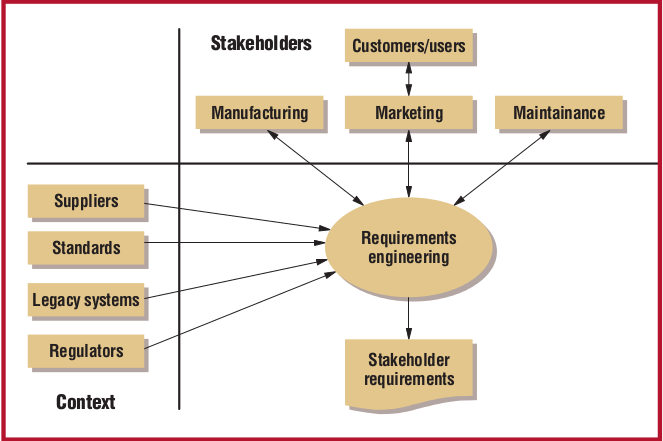
\includegraphics[scale=0.6]{stakeholder}
            \rule{35em}{0.5pt}
            \caption{Các bên yêu cầu (stakeholder) trong một dự án hệ thống nhúng}
            \label{fig:stakeholder}
        \end{figure}

        Bước đầu, khách hàng xác định các yêu cầu chức năng
        (\texttt{functional}) và các yêu cầu phi chức năng
        (\texttt{non-functional}). Tuỳ thuộc vào loại sản phẩm mà khách hàng sẽ
        đàm phán qua bộ phận marketing hay trực tiếp với các nhà phát triển.

        Kết quả của bước này sẽ là một bản đặc tả các yêu cầu, mô tả về hệ
        thống sao cho tất cả các bên yêu cầu đều có thể hiểu được. Tài liệu này
        được coi như hợp đồng với nhà phát triển (phần mềm nhúng).

        \paragraph{Đặc tả yêu cầu}

        Với phần mềm nhúng, các đặc tả phi chức năng (\texttt{non-functional
        specification}) rất quan trọng (do các ràng buộc về tài nguyên hạn chế,
        đáp ứng ở thời gian thực, mức tiêu thụ năng lượng, \ldots). Mà đặc tả
        phi chức năng thường rất khó phát biểu chính xác, do đó không
        thể dùng các phương pháp đặc tả yêu cầu như bình thường (như sử dụng
        các mẫu (template) của các trình soạn thảo văn bản).

        Với những dự án có sử dụng các biểu đồ để đặc tả, các biểu đồ này hầu
        hết ở dạng tự do hoặc các biểu đồ tương tự với UML, DFD
        (\texttt{Dataflow diagrams} - biểu đồ luồng dữ liệu), \ldots. Do không
        có một sự thống nhất về cú pháp của các biểu đồ, các thành viên dự án
        có thể hiểu sai ý nghĩa của nó.

        Đặc tả hình thức (\texttt{formal specification}) thường ít được sử
        dụng do tính phức tạp của hệ thống nhúng cũng như các yêu cầu của nó.
        Việc sử dụng đặc tả hình thức sẽ làm sự hợp tác giữa các thành viên
        trong dự án trở nên khó khăn hơn vì hầu hết các thành viên đều không
        hoàn toàn hiểu nó. Với khách hàng thì vấn đề này còn khó khăn hơn nữa.

%=============== Thiết kế ========================
    \section{Thiết kế}
        \subsection{Thiết kế hệ thống}
            Ở bước này, tổ chức tổng quát của chương trình sẽ được phát triển,
            bao gồm:
            \begin{itemize}
                \item Task: các tác vụ, 
                \item Comumunications:  sự liên lạc giữa các tác vụ với
            nhau cũng như giữa hệt thống và thể giới bên ngoài, 
                \item Timing:  sự phân bố thời gian trên toàn hệ thống, đảm bảo mỗi tác
                    vụ hoạt động trong đúng khoảng thời gian để hoàn thành chức
                    năng của nó,
                \item Priority: độ ưu tiên, để nhường quyền thực hiện cho một số tác vụ
                    nào đó được coi là quan trọng cho hệ thống vào một thời
                    điểm bất kỳ.
            \end{itemize}

            Đây là những yêu cầu cơ bản cho ứng dụng đa tác vụ. 

            Để bắt đầu thiết kế mức hệ thống, người thiết kế cần phải hiểu rõ
            chương trình cần phải hoàn thành những gì. Hay phải hiểu rõ được
            các yêu cầu của phần mềm.

            \subsubsection{Xác định các tác vụ}
                Đây là quá trình hợp các yêu cầu chức năng của phần mềm lại
                và hợp thành một số ít các tác vụ. Mỗi tác vụ sẽ là một module
                có thể được thực hiện riêng biệt, có Comumunications, Timing,
                Priority riêng của nó. Do đó, các chức năng bên trong module
                phải tương thích với nhau, hay ít nhất là có thể thực hiện hiện
                mà không ảnh hưởng đến chức năng khác.

                Các chức năng được coi là tương thích với nhau nếu thoả mãn một
                trong các tiêu chí sau \cite{EmbSysWD}:
                \begin{itemize}
                    \item Thực hiện tuần tự,
                    \item Thực hiện đồng bộ với nhau,
                    \item Cùng quản lý một thiết bị ngoại vì,
                    \item Quản lý dữ liệu chung,
                    \item Loại trừ lẫn nhau trong lúc thực hiện,
                    \item Đều là sự mở rộng của một chức năng khác.
                \end{itemize}

                Các chức năng thoả mãn một trong các tiêu chí sau đây thì được
                gọi là không tương thích với nhau. Không nên cho các chức năng
                này vào cùng một module.
                \begin{itemize}
                    \item Thực hiện không đồng bộ,
                    \item Thực hiện ở tốc độ (rate) khác nhau,
                    \item Có mức độ ưu tiên khác nhau
                \end{itemize}

            \subsubsection{Giao tiếp}
                Bước tiếp theo của thiết kế hệ thống là xác định các giao tiếp
                giữa các tác vụ với nhau và với thế giới bên ngoài (thông qua
                các thiết bị ngoại vi) của hệ thống. Qua bước này, chúng ta có
                thể:
                \begin{enumerate}
                    \item ước lượng được bộ nhớ cần thiết cho hệ thống,
                    \item Xác định tất cả các biến trong chương trình mà không
                        thuộc vào một tác vụ cụ thể nào,
                \end{enumerate}

                Người ta thường sử dụng biểu đồ luồng dữ liệu (DFD) để diễn tác
                các giao tiếp.

                \begin{figure}[H]
                    \centering
                    \includegraphics[scale=0.6]{dfdcom}
                    \rule{35em}{0.5pt}
                    \caption{Biểu đồ luồng dữ liệu cho đồng hồ báo thức}
                    \label{fig:dfdcom}
                \end{figure}

                Hình \ref{fig:dfdcom} là sơ đồ luồng dữ liệu biểu diễn giao
                tiếp giữa các tác vụ của một đồng hồ báo thức. Trong đó hình
                tròn biểu diễn cho một tác vụ, các đường thẳng chỉ ra giao tiếp
                giữa chúng.


        \subsection{Thiết kế chương trình}
            \paragraph{Thiết kế hướng đối tượng / hướng thủ tục}
                Các phương pháp thiết kế này sử dụng các \texttt{thủ tục} (đối với
                thiết kế hướng đối tượng là \texttt{phương thức}) là các thành
                phần cơ bản của chương trình. Các thủ tục (phương thức) này
                nhận các tham số, thực hiện một số hữu hạn các phép tính và trả
                về giá trị.

                Phương pháp hướng đối tượng hợp nhất các thủ tục và dữ liệu để
                tạo thành các \texttt{đối tượng (object)}. Các đối tượng này là
                thụ động, bởi vì nó cần sự tác động của bên ngoài để thực hiện
                các phương thức của nó.

                Tuy nhiên thế giới thực là chủ động, giống với các tiến trình
                hơn là các đối tượng, nó hoạt động trên các luồng riêng, tương
                tác với các tiến trình khác bằng các thông điệp. 

                Như vậy, mặc dù thiết kế hướng đối tượng được sử dụng rất nhiều
                trong việc xây dựng các hệ thống phần mèm lớn, nó lại không
                thích hợp cho việc giải quyết các vấn đề của việc thiết kế phần
                mềm nhúng.

                Người ta đã mở rộng mô hình thiết kế hướng đối tượng thành \texttt{mô
                hình hướng đối tượng thời gian thực (Realtime Object-Oriented
                Model - ROOM)} \cite{ROOM}. ROOM hỗ trợ UML-RT, một mở rộng của
                UML chuẩn dành cho các hệ thống thời gian thực. 

                \begin{figure}[H]
                    \centering
                    \includegraphics[scale=0.6]{umlrt}
                    \rule{35em}{0.5pt}
                    \caption{UML-RT}
                    \label{fig:umlrt}
                \end{figure}

                Hình \ref{fig:umlrt} minh hoạ cho biểu đồ UML-RT. Trong đó A, B
                là các \texttt{capsule} - đối tượng tích cực. Các capsule đều
                có các \texttt{port} để kết nối với nhau. Các capsule sẽ truyền
                thông điệp qua các port này.
                
%============ Coding =============================
    \section{Mã hoá chương trình}
        \paragraph{Ngôn ngữ lập trình}
            Do thường gặp hạn chế về tài nguyên cũng như yêu cầu về hiệu năng,
            C và Assembly là hai ngôn ngữ thường được sử dụng trong lập trình
            phần mềm nhúng. Chương trình viết bằng 2 ngôn ngữ này thường nhỏ,
            nhanh và có khả năng thao tác trực tiếp với phần cứng. Trong đó
            Assembly thường được dùng cho những nơi cần yêu cầu cao về hiệu
            năng, kích thước chương trình hay là phụ thuộc phần cứng (VD:
            driver).

            Mặc dù ngôn ngữ C không trực tiếp hỗ trợ lập trình hướng đối tượng
            nhưng vẫn có thể sử dụng các kỹ thuật hướng đối tượng bằng các cấu
            trúc có sẵn của C:
            \begin{itemize}
                \item Sử dụng struct thay cho class,
                \item Sử dụng hàm với đối số đầu kiểu của struct thay
                    cho phương thức,
                \item Sử dụng con trỏ void để có được khả năng đa hình,
                \item \ldots
            \end{itemize}


            Ngoài ra, cũng có thể dùng C++ cho phát triển phần mềm nhúng. C++
            kế thừa được những ưu điểm của C (mềm dẻo, hiệu năng) cộng thểm
            nhiều tính năng khác làm cho việc lập trình đơn giản hơn (template,
            STL, \ldots). Tuy vậy cần chú ý đến kích thước chương trình khi sử
            dụng các tính năng này. Ngoài ra một số tính năng như exception
            cũng có thể không được hỗ trợ trên một số hệ thống.

        \paragraph{Một số vấn đề khi mã hoá chương trình phần mềm nhúng}
            \subparagraph{Sự phụ thuộc nền tảng}
                Một chương trình có thể chạy đúng với phần cứng này, HDH này
                nhưng chưa chắc đã chạy đúng trên phần cứng, HDH khác. Đó là do
                một số yếu tố trong chương trình khác nhau ở những nền tảng
                khác nhau. Ví dụ:
                \begin{itemize}
                    \item Kích thước kiểu dữ liệu nguyên (\texttt{int, long,
                        short}, các
                        kiểu con trỏ): ngôn ngữ C/C++ không quy định về kích
                        thước chính xác của các kiểu dữ liệu này. VD: HDH 32bit
                        thường quy định kích thước con trỏ là 32bit, HDH 64bit
                        thường quy định kích thước con trỏ là 64bit. Do vậy cần
                        chú ý khi sử dụng các kiểu dữ liệu này, không nên mặc
                        nhiên coi rằng một kiểu dữ liệu nào đó có một kích
                        thước xác định. Nếu muốn kiểu nguyên với kích thước cụ
                        thể thì sử dụng các kiểu có sẵn như \texttt{int32\_t,
                        uint16\_t, \ldots}.
                    \item Sự căn chỉnh byte (byte alignment) và thứ tự byte
                        (byte order): Với mỗi hệ thống khác nhau, yêu cầu về
                        byte alignment và byte order có thể khác nhau. VD: trên
                        MIPS, truy cập vào một biến nguyên 32bit có địa chỉ
                        không chia hết cho 4 sẽ sinh ra lỗi SIGBUS.
                    \item Tính toán số thực dấu phẩy động: nhiều vi xử lý hiện nay
                        không hỗ trợ tính toán trên dấu phẩy động. Khi đưa
                        chương trình lên nền tảng này cần cân nhắc việc cài đặt
                        tính năng này bằng phần mềm hoặc sử dụng một thuật toán
                        khác không sử dụng đến tính toán số thực dấu phẩy động.
                \end{itemize}
            \subparagraph{Hạn chế về tài nguyên}
                Đây luôn là vấn đề xuyên suốt cả quá trình phát triển phần mềm
                nhúng. Trong gian đoạn mã hoá chương trình này, cần tuân thủ
                chặt chẽ các nguyên tắc để sự dụng tiết kiệm tài nguyên nhất có
                thể mà vẫn đảm bảo được hiệu năng.

        \paragraph{Công cụ}
            \subparagraph{Trình biên dịch (compiler)}
                Trình biên dịch được sử dụng trong lập trình nhúng là cross
                compiler, tức là trình dịch chạy trên host nhưng lại sinh mà
                cho target. Với mỗi target khác nhau sẽ có một cross compiler
                riêng, thường do các nhà sản xuất vi xử lý cung cấp. Ngoài ra
                còn có những trình biên dịch có thể sinh mã cho nhiều target
                khác nhau, như GCC hỗ trợ hơn 20 loại vi xử lý \cite{GccWiki}.

            \subparagraph{Trình dịch hợp ngữ (Assembler)}
                Chạy trên host. Có nhiệm vụ dịch mã hợp ngữ được sinh ra bởi
                compiler thành mã máy.

            \subparagraph{Trình liên kết (Linker)}
                Liên kết các file mã máy (nhị phân) đã được biên dịch cùng với
                các thư viện cần thiết thành chương trình hoàn chỉnh. Cũng chạy
                trên host.

            \subparagraph{Chương trình giả lập (emulator)}
                Giả lập target trên host. Dùng để debug hoặc test chương trình
                mà không cần phải sử dụng phần cứng thật (target). Emulator
                thường sử dụng phương pháp thông dịch mã nhị phân của target thành mã
                nhị phân dành cho máy host để máy host có thể hiểu và thực thi
                được chương trình. Do đó chương trình chạy trên emulator thường
                chậm hơn so với máy thực.


                \begin{figure}[H]
                    \centering
                    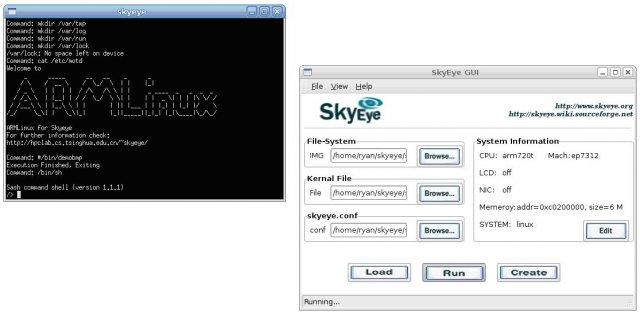
\includegraphics[scale=0.6]{armemu}
                    \rule{35em}{0.5pt}
                    \caption{Giả lập ARM trên PC x86}
                    \label{fig:armemu}
                \end{figure}

            \subsection{Môi trường phát triển tích hợp}
                Chương trình hợp nhất tất cả các công cụ phát triển (compiler, assembler,
                linker, emulator, \ldots).
                

                \begin{figure}[H]
                    \centering
                    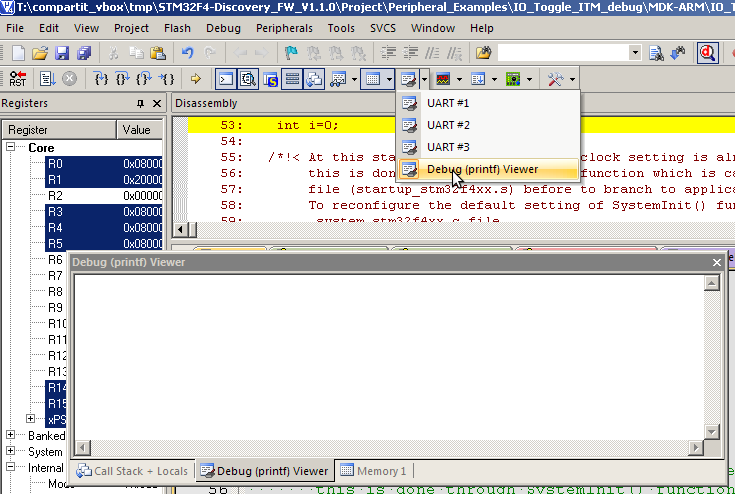
\includegraphics[scale=0.6]{keil}
                    \rule{35em}{0.5pt}
                    \caption{Keil - IDE phát triển phần mềm trên các vi xử lý họ ARM}
                    \label{fig:keil}
                \end{figure}

%================= Testing ===================================
    \section{Kiểm thử}
        Kiểm thử phần mềm nhúng có nhiều điểm giống nhau so với kiểm thử phần
        mềm ứng dụng thông thường. Tuy nhiên, có một vài điểm khác nhau giữa
        hai loại kiểm thử. Kiểm thử phần mềm nhúng thường phải truy cập đến
        những công cụ kiểm thử dựa trên phần cứng, cái thường không được sự
        dụng trong phát triển phần mềm ứng dụng.

        Kiểm thử cho điện thoại di động đương nhiên sẽ khác so với kiểm thử một
        bộ phận điều khiển của xe hơi. Mỗi công việc đều đòi hỏi định lượng
        pháp kiểm thử cho từng hệ thống riêng biệt. Không có một phương pháp
        chung nào cho tất cả các hệ thống nhúng.

        Quá trình kiểm thử phần mềm nhúng cơ bản như hình \ref{fig:embdevprg}.

        \begin{figure}[H]
            \centering
            \includegraphics[scale=0.6]{embdevprg}
            \rule{35em}{0.5pt}
            \caption{Quy trình kiểm thử phần mềm nhúng}
            \label{fig:embdevprg}
        \end{figure}

        Như đã nói trước đó, phần mềm nhúng thường phát triển song song cùng
        lúc với phần cứng. Kiểm thử phần mềm nhúng phải đi đôi với kiểm thử
        phần cứng.

        \subsection{Các giai đoạn kiểm thử}
            \begin{enumerate}
                \item Kiểm thử module
                \item Kiểm thử tích hợp
                \item Kiểm thử hệ thống (phần mềm)
                \item Kiểm thử tích hợp phần cứng - phần mềm
            \end{enumerate}
            Như vậy, so với kiểm thử thông thường thì kiểm thử phần mềm nhúng
            có thêm giai đoạn kiểm thử tích hợp phần cứng - phần mềm.

        \subsection{Kiểm thử trên môi trường giả lập}
            Trước khi chạy trên máy thật, phần mềm nhúng được kiểm thử trên môi
            trường giả lập chạy trên máy host. Ưu điểm của phương pháp này là
            cài đặt đơn giản (đơn giản hơn so với việc đưa chương trình lên máy
            thật), tiết kiệm, có khả năng tùy biến cao.

        \subsection{Kiểm thử trên thiết bị thật}
            Các môi trường giả lập trên PC không phải lúc nào cũng có thể giả lập được
            hết các tính năng của thiết bị, VD: tính năng rung trên điện thoại
            di động, định vị GPS, \ldots. Và cũng không thể hiện được hết tất
            cả các tình huống có thể gặp phải trong thế giới thật, VD: các sự
            kiện xảy ra đồng thời. Ngoài ra, hiệu năng của chương trình trên
            môi trường giả lập cũng không giống với trên thiết bị thật (thường
            là chậm hơn), do đó không thể đánh giá đúng được hiệu năng thật
            (vốn là một yếu tố rất quan trọng của phần mềm nhúng).

            Do vậy, cần phải kiểm thử trên thiết bị thật. Chỉ khi nào chương
            trình chạy đúng trên thiết bị thật thì mới được coi là kiểm thử hoàn thành.

        \subsection{Một số vấn đề trong kiểm thử phần mềm nhúng}
            \begin{itemize}
                \item Kiểm thử các hệ thống thời gian thực khó bởi vì chúng
                    phản ứng với các sự kiện và dữ liệu không đồng bộ. Trên
                    thực tế gần như không thể kiểm tra một cách toàn diện các
                    trường hợp đầu vào của một hệ thống nhúng.

                \item Không thể sử dụng các phương pháp kiểm thử thông thường
                    vào một số hệ thống (vì dụ: không thể đặt breakpoint trong
                    quá trình thực thi hệ thống điều khiển máy bay khi nó đang
                    ở độ cao hàng chục km!). Nếu những hệ thống này hoạt động
                    sai, gần như không thể lặp lại chuỗi sự kiện dẫn đển lỗi để
                    tìm cách chẩn đoán.

                \item Nhiều hệ thống phụ thuộc vào trạng thái, có nghĩa là phản
                    ứng đối với một sự kiện không chỉ phụ thuộc vào sự kiện đó
                    mà còn phụ thuộc vào những gì đã xảy ra trước đó. Nói cách
                    khác, hai sự kiện giống nhau có thể dẫn đến kết quả khác
                    nhau.
            \end{itemize}

%================= Maintenance ==============================
    \section{Bảo trì}
        Về cơ bản, bảo trì phần mềm nhúng không khác với bảo trì phần mềm thông
        thường. Chúng đều có các bước chính như nhau. Tuy nhiên, do các đặc
        tính của phần mềm nhúng mà có một số yếu tố phát sinh \cite{EmbMtn}.

        \paragraph{Một số vấn đề trong bảo trì phần mềm nhúng}
            
            \begin{itemize}
                \item Các yêu cầu không ổn định:
                    Với phần mềm nhúng, các yêu cầu đuợc thêm vào và thay đổi
                    thường xuyên. Sự thay đổi thường không phải lúc nào cũng
                    có thể thông báo được đến tất cả các bên. Do đó việc bảo trì
                    trở nên rất phức tạp.

                \item Sự thay đổi về công nghệ:
                    Công nghệ phần cứng thường phát triển nhanh hơn phần mềm.

                \item Cần phải đào tạo:
                    Với một vài lĩnh vực, quá trình bảo trì phức tạp bởi rất khó để
                    hiểu được chương trình phần mềm. 

                \item Môi trường giả lập vs thiết bị thực (target):
                    Thông thường, những người phát triển phần mềm không phải ai
                    cũng có quyền tiếp xúc với thiết bị thực, việc phát triển /
                    bảo trì
                    phần mềm trở nên phụ thuộc vào môi trường giả lập.

                \item Ràng buộc về phần cứng
            \end{itemize} 
        
                
 % ANN
%\input{./Chapters/Chapter4} % Chương trình demo

%\chapter{Quy trình phát triển phần mềm}
    \section{Định nghĩa}
        Toàn bộ quy trình quản lý phát triển phần mềm gắn với khái niệm vòng đời phần mềm, được mô hình hóa với những kỹ thuật và phương pháp luận trở thành các chủ đề khác nhau trong Công nghệ phần mềm.

        \paragraph{Vòng đời của phần mềm} là thời kì tính từ khi phần mêm được
        bắt đầu sinh ra cho đến khi chết đi (từ lúc hình thành đáp ứng yêu cầu,
        vận hành, bảo dưỡng cho đến khi loại bỏ không dùng nữa),

        \paragraph{Chuẩn ISO/IEC 12207:2008} là một chuẩn quốc tế về quy trình phát triển phần
        mềm, định nghĩa tất cả các công việc cần thiết cho việc phát triển và
        bảo trì phần mềm \cite{ISOWiki}.

        Chuẩn ISO/IEC 12207:2008 quy định 43 quá trình (process), trong đó có
        các pha chính là: 
            \begin{itemize}
                \item phân tích/xác định yêu cầu người dùng, 
                \item thiết kế, 
                \item mã hoá, 
                \item kiểm thử, 
                \item bảo trì.
            \end{itemize}

        \paragraph{Mô hình phát triển phần mềm} sắp xếp các quá trình phát
        triển phần mềm theo một cách nào đó. Có nhiều mô hình phát triển phần
        mềm khác nhau, mỗi cái đều có ưu và nhược điểm riêng. Có thể kể đến:
        \begin{itemize}
            \item Mô hình thác nước (Waterfall model),
            \item Mô hình xoắn ốc (Spiral model),
            \item Mô hình lập trình linh hoạt (agile development),
            \item Mô hình chế thử (prototype model),
            \item \ldots
        \end{itemize}

    \section{Các quá trình trong phát triển phần mềm}
        \subsection{Phân tích - xác định yêu cầu}
        
        \subsection{Thiết kế}

    \section{Một số mô hình phát triển phần mềm}
        \subsection{Mô hình thác nước}
 % Background Theory 

%\chapter{Quy trình phát triển phần mềm nhúng}
    

%================ Requirement ===================
    \section{Xác định yêu cầu người dùng}
        Việc phát triển một hệ thống nhúng thường có nhiều người yêu cầu, bao
        gồm: nhà sản xuất phần cứng, người bảo trì, marketing, khách hàng (hình
        \ref{fig:stakeholder})\cite{EmbSysState}.

        \begin{figure}[H]
            \centering
            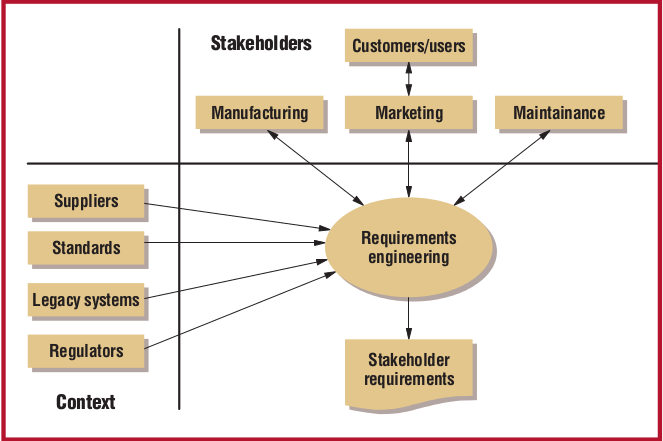
\includegraphics[scale=0.6]{stakeholder}
            \rule{35em}{0.5pt}
            \caption{Các bên yêu cầu (stakeholder) trong một dự án hệ thống nhúng}
            \label{fig:stakeholder}
        \end{figure}

        Bước đầu, khách hàng xác định các yêu cầu chức năng
        (\texttt{functional}) và các yêu cầu phi chức năng
        (\texttt{non-functional}). Tuỳ thuộc vào loại sản phẩm mà khách hàng sẽ
        đàm phán qua bộ phận marketing hay trực tiếp với các nhà phát triển.

        Kết quả của bước này sẽ là một bản đặc tả các yêu cầu, mô tả về hệ
        thống sao cho tất cả các bên yêu cầu đều có thể hiểu được. Tài liệu này
        được coi như hợp đồng với nhà phát triển (phần mềm nhúng).

        \paragraph{Đặc tả yêu cầu}

        Với phần mềm nhúng, các đặc tả phi chức năng (\texttt{non-functional
        specification}) rất quan trọng (do các ràng buộc về tài nguyên hạn chế,
        đáp ứng ở thời gian thực, mức tiêu thụ năng lượng, \ldots). Mà đặc tả
        phi chức năng thường rất khó phát biểu chính xác, do đó không
        thể dùng các phương pháp đặc tả yêu cầu như bình thường (như sử dụng
        các mẫu (template) của các trình soạn thảo văn bản).

        Với những dự án có sử dụng các biểu đồ để đặc tả, các biểu đồ này hầu
        hết ở dạng tự do hoặc các biểu đồ tương tự với UML, DFD
        (\texttt{Dataflow diagrams} - biểu đồ luồng dữ liệu), \ldots. Do không
        có một sự thống nhất về cú pháp của các biểu đồ, các thành viên dự án
        có thể hiểu sai ý nghĩa của nó.

        Đặc tả hình thức (\texttt{formal specification}) thường ít được sử
        dụng do tính phức tạp của hệ thống nhúng cũng như các yêu cầu của nó.
        Việc sử dụng đặc tả hình thức sẽ làm sự hợp tác giữa các thành viên
        trong dự án trở nên khó khăn hơn vì hầu hết các thành viên đều không
        hoàn toàn hiểu nó. Với khách hàng thì vấn đề này còn khó khăn hơn nữa.

%=============== Thiết kế ========================
    \section{Thiết kế}
        \subsection{Thiết kế hệ thống}
            Ở bước này, tổ chức tổng quát của chương trình sẽ được phát triển,
            bao gồm:
            \begin{itemize}
                \item Task: các tác vụ, 
                \item Comumunications:  sự liên lạc giữa các tác vụ với
            nhau cũng như giữa hệt thống và thể giới bên ngoài, 
                \item Timing:  sự phân bố thời gian trên toàn hệ thống, đảm bảo mỗi tác
                    vụ hoạt động trong đúng khoảng thời gian để hoàn thành chức
                    năng của nó,
                \item Priority: độ ưu tiên, để nhường quyền thực hiện cho một số tác vụ
                    nào đó được coi là quan trọng cho hệ thống vào một thời
                    điểm bất kỳ.
            \end{itemize}

            Đây là những yêu cầu cơ bản cho ứng dụng đa tác vụ. 

            Để bắt đầu thiết kế mức hệ thống, người thiết kế cần phải hiểu rõ
            chương trình cần phải hoàn thành những gì. Hay phải hiểu rõ được
            các yêu cầu của phần mềm.

            \subsubsection{Xác định các tác vụ}
                Đây là quá trình hợp các yêu cầu chức năng của phần mềm lại
                và hợp thành một số ít các tác vụ. Mỗi tác vụ sẽ là một module
                có thể được thực hiện riêng biệt, có Comumunications, Timing,
                Priority riêng của nó. Do đó, các chức năng bên trong module
                phải tương thích với nhau, hay ít nhất là có thể thực hiện hiện
                mà không ảnh hưởng đến chức năng khác.

                Các chức năng được coi là tương thích với nhau nếu thoả mãn một
                trong các tiêu chí sau \cite{EmbSysWD}:
                \begin{itemize}
                    \item Thực hiện tuần tự,
                    \item Thực hiện đồng bộ với nhau,
                    \item Cùng quản lý một thiết bị ngoại vì,
                    \item Quản lý dữ liệu chung,
                    \item Loại trừ lẫn nhau trong lúc thực hiện,
                    \item Đều là sự mở rộng của một chức năng khác.
                \end{itemize}

                Các chức năng thoả mãn một trong các tiêu chí sau đây thì được
                gọi là không tương thích với nhau. Không nên cho các chức năng
                này vào cùng một module.
                \begin{itemize}
                    \item Thực hiện không đồng bộ,
                    \item Thực hiện ở tốc độ (rate) khác nhau,
                    \item Có mức độ ưu tiên khác nhau
                \end{itemize}

            \subsubsection{Giao tiếp}
                Bước tiếp theo của thiết kế hệ thống là xác định các giao tiếp
                giữa các tác vụ với nhau và với thế giới bên ngoài (thông qua
                các thiết bị ngoại vi) của hệ thống. Qua bước này, chúng ta có
                thể:
                \begin{enumerate}
                    \item ước lượng được bộ nhớ cần thiết cho hệ thống,
                    \item Xác định tất cả các biến trong chương trình mà không
                        thuộc vào một tác vụ cụ thể nào,
                \end{enumerate}

                Người ta thường sử dụng biểu đồ luồng dữ liệu (DFD) để diễn tác
                các giao tiếp.

                \begin{figure}[H]
                    \centering
                    \includegraphics[scale=0.6]{dfdcom}
                    \rule{35em}{0.5pt}
                    \caption{Biểu đồ luồng dữ liệu cho đồng hồ báo thức}
                    \label{fig:dfdcom}
                \end{figure}

                Hình \ref{fig:dfdcom} là sơ đồ luồng dữ liệu biểu diễn giao
                tiếp giữa các tác vụ của một đồng hồ báo thức. Trong đó hình
                tròn biểu diễn cho một tác vụ, các đường thẳng chỉ ra giao tiếp
                giữa chúng.


        \subsection{Thiết kế chương trình}
            \paragraph{Thiết kế hướng đối tượng / hướng thủ tục}
                Các phương pháp thiết kế này sử dụng các \texttt{thủ tục} (đối với
                thiết kế hướng đối tượng là \texttt{phương thức}) là các thành
                phần cơ bản của chương trình. Các thủ tục (phương thức) này
                nhận các tham số, thực hiện một số hữu hạn các phép tính và trả
                về giá trị.

                Phương pháp hướng đối tượng hợp nhất các thủ tục và dữ liệu để
                tạo thành các \texttt{đối tượng (object)}. Các đối tượng này là
                thụ động, bởi vì nó cần sự tác động của bên ngoài để thực hiện
                các phương thức của nó.

                Tuy nhiên thế giới thực là chủ động, giống với các tiến trình
                hơn là các đối tượng, nó hoạt động trên các luồng riêng, tương
                tác với các tiến trình khác bằng các thông điệp. 

                Như vậy, mặc dù thiết kế hướng đối tượng được sử dụng rất nhiều
                trong việc xây dựng các hệ thống phần mèm lớn, nó lại không
                thích hợp cho việc giải quyết các vấn đề của việc thiết kế phần
                mềm nhúng.

                Người ta đã mở rộng mô hình thiết kế hướng đối tượng thành \texttt{mô
                hình hướng đối tượng thời gian thực (Realtime Object-Oriented
                Model - ROOM)} \cite{ROOM}. ROOM hỗ trợ UML-RT, một mở rộng của
                UML chuẩn dành cho các hệ thống thời gian thực. 

                \begin{figure}[H]
                    \centering
                    \includegraphics[scale=0.6]{umlrt}
                    \rule{35em}{0.5pt}
                    \caption{UML-RT}
                    \label{fig:umlrt}
                \end{figure}

                Hình \ref{fig:umlrt} minh hoạ cho biểu đồ UML-RT. Trong đó A, B
                là các \texttt{capsule} - đối tượng tích cực. Các capsule đều
                có các \texttt{port} để kết nối với nhau. Các capsule sẽ truyền
                thông điệp qua các port này.
                
%============ Coding =============================
    \section{Mã hoá chương trình}
        \paragraph{Ngôn ngữ lập trình}
            Do thường gặp hạn chế về tài nguyên cũng như yêu cầu về hiệu năng,
            C và Assembly là hai ngôn ngữ thường được sử dụng trong lập trình
            phần mềm nhúng. Chương trình viết bằng 2 ngôn ngữ này thường nhỏ,
            nhanh và có khả năng thao tác trực tiếp với phần cứng. Trong đó
            Assembly thường được dùng cho những nơi cần yêu cầu cao về hiệu
            năng, kích thước chương trình hay là phụ thuộc phần cứng (VD:
            driver).

            Mặc dù ngôn ngữ C không trực tiếp hỗ trợ lập trình hướng đối tượng
            nhưng vẫn có thể sử dụng các kỹ thuật hướng đối tượng bằng các cấu
            trúc có sẵn của C:
            \begin{itemize}
                \item Sử dụng struct thay cho class,
                \item Sử dụng hàm với đối số đầu kiểu của struct thay
                    cho phương thức,
                \item Sử dụng con trỏ void để có được khả năng đa hình,
                \item \ldots
            \end{itemize}


            Ngoài ra, cũng có thể dùng C++ cho phát triển phần mềm nhúng. C++
            kế thừa được những ưu điểm của C (mềm dẻo, hiệu năng) cộng thểm
            nhiều tính năng khác làm cho việc lập trình đơn giản hơn (template,
            STL, \ldots). Tuy vậy cần chú ý đến kích thước chương trình khi sử
            dụng các tính năng này. Ngoài ra một số tính năng như exception
            cũng có thể không được hỗ trợ trên một số hệ thống.

        \paragraph{Một số vấn đề khi mã hoá chương trình phần mềm nhúng}
            \subparagraph{Sự phụ thuộc nền tảng}
                Một chương trình có thể chạy đúng với phần cứng này, HDH này
                nhưng chưa chắc đã chạy đúng trên phần cứng, HDH khác. Đó là do
                một số yếu tố trong chương trình khác nhau ở những nền tảng
                khác nhau. Ví dụ:
                \begin{itemize}
                    \item Kích thước kiểu dữ liệu nguyên (\texttt{int, long,
                        short}, các
                        kiểu con trỏ): ngôn ngữ C/C++ không quy định về kích
                        thước chính xác của các kiểu dữ liệu này. VD: HDH 32bit
                        thường quy định kích thước con trỏ là 32bit, HDH 64bit
                        thường quy định kích thước con trỏ là 64bit. Do vậy cần
                        chú ý khi sử dụng các kiểu dữ liệu này, không nên mặc
                        nhiên coi rằng một kiểu dữ liệu nào đó có một kích
                        thước xác định. Nếu muốn kiểu nguyên với kích thước cụ
                        thể thì sử dụng các kiểu có sẵn như \texttt{int32\_t,
                        uint16\_t, \ldots}.
                    \item Sự căn chỉnh byte (byte alignment) và thứ tự byte
                        (byte order): Với mỗi hệ thống khác nhau, yêu cầu về
                        byte alignment và byte order có thể khác nhau. VD: trên
                        MIPS, truy cập vào một biến nguyên 32bit có địa chỉ
                        không chia hết cho 4 sẽ sinh ra lỗi SIGBUS.
                    \item Tính toán số thực dấu phẩy động: nhiều vi xử lý hiện nay
                        không hỗ trợ tính toán trên dấu phẩy động. Khi đưa
                        chương trình lên nền tảng này cần cân nhắc việc cài đặt
                        tính năng này bằng phần mềm hoặc sử dụng một thuật toán
                        khác không sử dụng đến tính toán số thực dấu phẩy động.
                \end{itemize}
            \subparagraph{Hạn chế về tài nguyên}
                Đây luôn là vấn đề xuyên suốt cả quá trình phát triển phần mềm
                nhúng. Trong gian đoạn mã hoá chương trình này, cần tuân thủ
                chặt chẽ các nguyên tắc để sự dụng tiết kiệm tài nguyên nhất có
                thể mà vẫn đảm bảo được hiệu năng.

        \paragraph{Công cụ}
            \subparagraph{Trình biên dịch (compiler)}
                Trình biên dịch được sử dụng trong lập trình nhúng là cross
                compiler, tức là trình dịch chạy trên host nhưng lại sinh mà
                cho target. Với mỗi target khác nhau sẽ có một cross compiler
                riêng, thường do các nhà sản xuất vi xử lý cung cấp. Ngoài ra
                còn có những trình biên dịch có thể sinh mã cho nhiều target
                khác nhau, như GCC hỗ trợ hơn 20 loại vi xử lý \cite{GccWiki}.

            \subparagraph{Trình dịch hợp ngữ (Assembler)}
                Chạy trên host. Có nhiệm vụ dịch mã hợp ngữ được sinh ra bởi
                compiler thành mã máy.

            \subparagraph{Trình liên kết (Linker)}
                Liên kết các file mã máy (nhị phân) đã được biên dịch cùng với
                các thư viện cần thiết thành chương trình hoàn chỉnh. Cũng chạy
                trên host.

            \subparagraph{Chương trình giả lập (emulator)}
                Giả lập target trên host. Dùng để debug hoặc test chương trình
                mà không cần phải sử dụng phần cứng thật (target). Emulator
                thường sử dụng phương pháp thông dịch mã nhị phân của target thành mã
                nhị phân dành cho máy host để máy host có thể hiểu và thực thi
                được chương trình. Do đó chương trình chạy trên emulator thường
                chậm hơn so với máy thực.


                \begin{figure}[H]
                    \centering
                    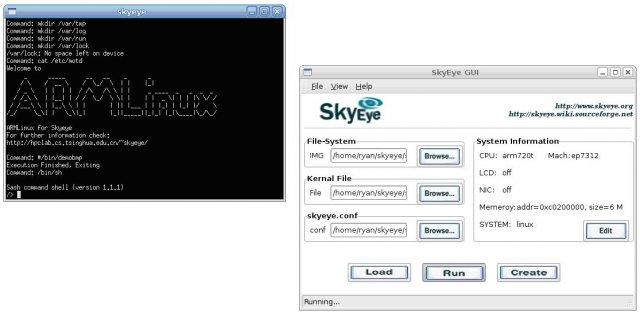
\includegraphics[scale=0.6]{armemu}
                    \rule{35em}{0.5pt}
                    \caption{Giả lập ARM trên PC x86}
                    \label{fig:armemu}
                \end{figure}

            \subsection{Môi trường phát triển tích hợp}
                Chương trình hợp nhất tất cả các công cụ phát triển (compiler, assembler,
                linker, emulator, \ldots).
                

                \begin{figure}[H]
                    \centering
                    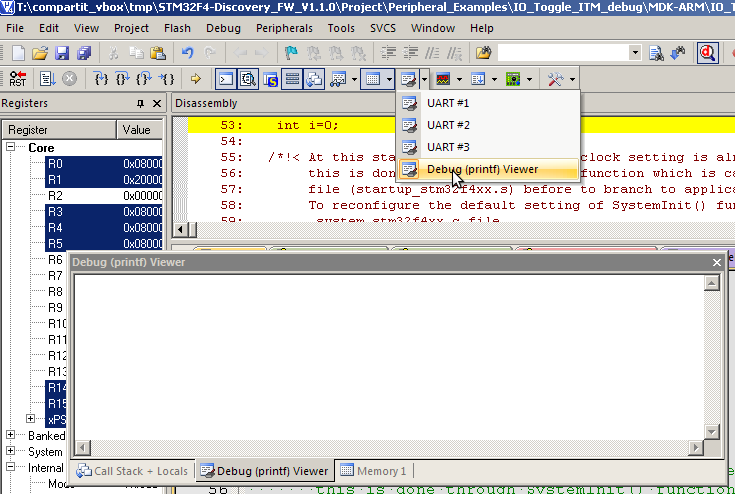
\includegraphics[scale=0.6]{keil}
                    \rule{35em}{0.5pt}
                    \caption{Keil - IDE phát triển phần mềm trên các vi xử lý họ ARM}
                    \label{fig:keil}
                \end{figure}

%================= Testing ===================================
    \section{Kiểm thử}
        Kiểm thử phần mềm nhúng có nhiều điểm giống nhau so với kiểm thử phần
        mềm ứng dụng thông thường. Tuy nhiên, có một vài điểm khác nhau giữa
        hai loại kiểm thử. Kiểm thử phần mềm nhúng thường phải truy cập đến
        những công cụ kiểm thử dựa trên phần cứng, cái thường không được sự
        dụng trong phát triển phần mềm ứng dụng.

        Kiểm thử cho điện thoại di động đương nhiên sẽ khác so với kiểm thử một
        bộ phận điều khiển của xe hơi. Mỗi công việc đều đòi hỏi định lượng
        pháp kiểm thử cho từng hệ thống riêng biệt. Không có một phương pháp
        chung nào cho tất cả các hệ thống nhúng.

        Quá trình kiểm thử phần mềm nhúng cơ bản như hình \ref{fig:embdevprg}.

        \begin{figure}[H]
            \centering
            \includegraphics[scale=0.6]{embdevprg}
            \rule{35em}{0.5pt}
            \caption{Quy trình kiểm thử phần mềm nhúng}
            \label{fig:embdevprg}
        \end{figure}

        Như đã nói trước đó, phần mềm nhúng thường phát triển song song cùng
        lúc với phần cứng. Kiểm thử phần mềm nhúng phải đi đôi với kiểm thử
        phần cứng.

        \subsection{Các giai đoạn kiểm thử}
            \begin{enumerate}
                \item Kiểm thử module
                \item Kiểm thử tích hợp
                \item Kiểm thử hệ thống (phần mềm)
                \item Kiểm thử tích hợp phần cứng - phần mềm
            \end{enumerate}
            Như vậy, so với kiểm thử thông thường thì kiểm thử phần mềm nhúng
            có thêm giai đoạn kiểm thử tích hợp phần cứng - phần mềm.

        \subsection{Kiểm thử trên môi trường giả lập}
            Trước khi chạy trên máy thật, phần mềm nhúng được kiểm thử trên môi
            trường giả lập chạy trên máy host. Ưu điểm của phương pháp này là
            cài đặt đơn giản (đơn giản hơn so với việc đưa chương trình lên máy
            thật), tiết kiệm, có khả năng tùy biến cao.

        \subsection{Kiểm thử trên thiết bị thật}
            Các môi trường giả lập trên PC không phải lúc nào cũng có thể giả lập được
            hết các tính năng của thiết bị, VD: tính năng rung trên điện thoại
            di động, định vị GPS, \ldots. Và cũng không thể hiện được hết tất
            cả các tình huống có thể gặp phải trong thế giới thật, VD: các sự
            kiện xảy ra đồng thời. Ngoài ra, hiệu năng của chương trình trên
            môi trường giả lập cũng không giống với trên thiết bị thật (thường
            là chậm hơn), do đó không thể đánh giá đúng được hiệu năng thật
            (vốn là một yếu tố rất quan trọng của phần mềm nhúng).

            Do vậy, cần phải kiểm thử trên thiết bị thật. Chỉ khi nào chương
            trình chạy đúng trên thiết bị thật thì mới được coi là kiểm thử hoàn thành.

        \subsection{Một số vấn đề trong kiểm thử phần mềm nhúng}
            \begin{itemize}
                \item Kiểm thử các hệ thống thời gian thực khó bởi vì chúng
                    phản ứng với các sự kiện và dữ liệu không đồng bộ. Trên
                    thực tế gần như không thể kiểm tra một cách toàn diện các
                    trường hợp đầu vào của một hệ thống nhúng.

                \item Không thể sử dụng các phương pháp kiểm thử thông thường
                    vào một số hệ thống (vì dụ: không thể đặt breakpoint trong
                    quá trình thực thi hệ thống điều khiển máy bay khi nó đang
                    ở độ cao hàng chục km!). Nếu những hệ thống này hoạt động
                    sai, gần như không thể lặp lại chuỗi sự kiện dẫn đển lỗi để
                    tìm cách chẩn đoán.

                \item Nhiều hệ thống phụ thuộc vào trạng thái, có nghĩa là phản
                    ứng đối với một sự kiện không chỉ phụ thuộc vào sự kiện đó
                    mà còn phụ thuộc vào những gì đã xảy ra trước đó. Nói cách
                    khác, hai sự kiện giống nhau có thể dẫn đến kết quả khác
                    nhau.
            \end{itemize}

%================= Maintenance ==============================
    \section{Bảo trì}
        Về cơ bản, bảo trì phần mềm nhúng không khác với bảo trì phần mềm thông
        thường. Chúng đều có các bước chính như nhau. Tuy nhiên, do các đặc
        tính của phần mềm nhúng mà có một số yếu tố phát sinh \cite{EmbMtn}.

        \paragraph{Một số vấn đề trong bảo trì phần mềm nhúng}
            
            \begin{itemize}
                \item Các yêu cầu không ổn định:
                    Với phần mềm nhúng, các yêu cầu đuợc thêm vào và thay đổi
                    thường xuyên. Sự thay đổi thường không phải lúc nào cũng
                    có thể thông báo được đến tất cả các bên. Do đó việc bảo trì
                    trở nên rất phức tạp.

                \item Sự thay đổi về công nghệ:
                    Công nghệ phần cứng thường phát triển nhanh hơn phần mềm.

                \item Cần phải đào tạo:
                    Với một vài lĩnh vực, quá trình bảo trì phức tạp bởi rất khó để
                    hiểu được chương trình phần mềm. 

                \item Môi trường giả lập vs thiết bị thực (target):
                    Thông thường, những người phát triển phần mềm không phải ai
                    cũng có quyền tiếp xúc với thiết bị thực, việc phát triển /
                    bảo trì
                    phần mềm trở nên phụ thuộc vào môi trường giả lập.

                \item Ràng buộc về phần cứng
            \end{itemize} 
        
                
 % Experimental Setup

%\input{./Chapters/Chapter4} % Experiment 1

%\input{./Chapters/Chapter5} % Experiment 2

%\input{./Chapters/Chapter6} % Results and Discussion

%\input{./Chapters/Chapter7} % Conclusion

%% ----------------------------------------------------------------
% Now begin the Appendices, including them as separate files

\addtocontents{toc}{\vspace{2em}} % Add a gap in the Contents, for aesthetics

%\appendix % Cue to tell LaTeX that the following 'chapters' are Appendices

%\input{./Appendices/AppendixA}	% Appendix Title

%\input{./Appendices/AppendixB} % Appendix Title

%\input{./Appendices/AppendixC} % Appendix Title

\addtocontents{toc}{\vspace{2em}}  % Add a gap in the Contents, for aesthetics
\backmatter

%% ----------------------------------------------------------------
\label{Bibliography}
\lhead{\emph{Bibliography}}  % Change the left side page header to "Bibliography"
\bibliographystyle{unsrtnat}  % Use the "unsrtnat" BibTeX style for formatting the Bibliography
\bibliography{Bibliography}  % The references (bibliography) information are stored in the file named "Bibliography.bib"

\end{document}  % The End
%% ----------------------------------------------------------------
